%This chapter presents the context, motivation and PhD framework railways WSN-based smart grid. 

\section{Context and motivation for PhD}

The railway system is responsible for 1.3\% of entire European energy consumption, \cite{iea-uic2016}. 
The debate on energy efficiency in railways is a well-discussed topic thanks to its impact on global energy consumption.

%The energy efficiency analysis and management 
Analysis and management of energy efficiency requires a detailed mapping of energy consumption/generation in the railway system. 
This detailed mapping of the energy flows must include, not only the rolling stock level but also the traction substations and the auxiliary services.
The knowledge of all the load curves permits load prevision, peak shaving and energy cost optimization of the railway system.


\section{Shift2Rail Framework}

This work is supported by the iRail PhD program – Innovation in Railway Systems and Technologies whose objectives are aligned with the \ac{S2R} objectives, \cite{shift2rail2015}, namely: 

\begin{itemize}
	\setlength\itemsep{-0.5em}
	\item 1. Cutting the life-cycle cost of railway transport by, at least, 50\%;
	\item 2. Doubling the railway capacity;
	\item 3. Increasing the reliability and punctuality by 50\%, at least.
\end{itemize}

In addition, the time target goals are the establishment of a framework, by 2020, for an European multimodal transport system for the passenger rail, freight and for the urban mobility. By 2030 is expected to triple the length of the existing high-speed passenger rail network and is expected to increase 30\% of the road freight over 300 km should shift to rail or waterborne transport to achieve a CO2-free city logistics in major urban centers. By 2050, the medium-distance passenger transport should move by rail and high-speed rail, and a connection should be achieved with all core network airports and the high-speed railway network. 
At the same time, by 2050, it should be expected that all seaports would be connected to the rail freight transport system and the urban mobility would be improved with the elimination of the "conventionally-fueled" cars from cities, \cite{shift2rail2015}.

%On the freight is expected to have all seaports connected to the rail freight transport system and on the urban mobility, the "conventionally-fueled" cars will not have place in cities by 2050, \cite{shift2rail2015}.


The \ac{S2R} carries five innovation programmes, as presented in figure \ref{fig:ips}. Framed on the S2R \ac{IP3} with the focus on the ”Cost efficient and reliable infrastructure”, it is proposed the development of a \ac{SMD} that achieves a detailed monitoring and supervision for various energy flows on the premises of embracing the entire \ac{RTS}.

\begin{figure}[h!]
	\centering
	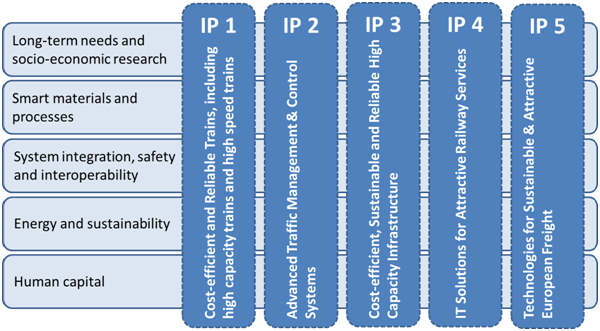
\includegraphics[width=0.60\textwidth,keepaspectratio]{figures/1.Intro/IPs}
	\caption{Shif2Rail Innovation Programs. Adapted from  \cite{shift2rail2015}.}
	\label{fig:ips}
\end{figure}

The purpose of any energy management strategy is build up on the dynamics of every loads and generators of the power system. 
This should be performed based on an extensive knowledge of every energy flows. 
Therefore, the \ac{SMD} is required to propose and validate a standard metering architecture that involves the coordination of every measurement performed either in on-board and in ground. 
In addition, energy data analysis should be provided based on relevant stored data. 

\section{Preliminary state of the art}

This section will cover a summary of the state of the art that supports this PhD.

Presently, the current metering systems focus on rolling stock on-board energy meters for energy billing purposes only, being located close to the pantograph, \cite{shift2rail2015}.
A possible advancement beyond the state of the art is the expansion of the measurement system to railway system level, making it a distributed on-board and track-side measurements, thus achieving detailed mappings. 

%\vspace{2em}

The analysis of the state of the art revealed a relevant level of intrusion in currently used metering systems, that in a way, became a critical subsystem of the rolling stock but also requires a relatively long implementation, \cite{shift2rail2015}. 
A solution based on non-intrusive technology appears to be a promising advancement. More detailed simulation models in conjunction with field measurements will be included on the methodology to be investigated.



%\textbf{\textit{Research Plan}}

A more challenging requirement to this research would be the development of non-intrusive  \ac{WSN}  in the railway environment. 
It is intended that this technology should be based on an open system and open interfaces for the data collection, aggregation and analysis. 
Issues like metering redundancy, outlier detection, fault tolerance and communication reliability, would be considered during the research.
In addition, it is expected the design and specification of a set of user applications.
Those applications are focused in the energy analysis process, with the aim of providing more information and detailed knowledge.
Ultimately, this detailed knowledge will be useful in a decision support system related with, in e.g., eco-driving strategies, timetable planning and preventive maintenance.

\newpage

\section{Document structure}

This document is divided in 5 chapters, each of them incorporating the relevant subsections to present the subjects mentioned. 
%contains several subsections according to the subjects mentioned.

\begin{table}[!h]
	\label{tb:struct}
	\centering
	\caption{Document structure}
	\vspace{0.2em}
	\begin{tabular}{c|l}%{C{2cm}|C{9cm}}
		\textbf{Chapter} & \textbf{Title}                    \\ \hline
		1       &                   Introduction             \\ \hline
		%  2       &                   Railways Remote Monitoring Systems       \\ \hline
		2       &                   Objectives and Contributions    \\ \hline
		3       &                   Literature Review    \\ \hline
		4       &                   Methodology and Work Plan       \\ \hline
		5       &                   Preliminary Work       \\
	\end{tabular}
\end{table}